\documentclass[11pt]{report}

% Paquetes y configuraciones adicionales
\usepackage[spanish]{babel} % Cargar el paquete babel con la opción en español
\usepackage{graphicx}
\usepackage[export]{adjustbox}
\usepackage{caption}
\usepackage{float}
\usepackage{titlesec}
\usepackage{geometry}
\usepackage[hidelinks]{hyperref}
\usepackage{parskip}
\usepackage{hyperref}
\usepackage{nameref}
\usepackage{listings}
\usepackage{wrapfig}
\usepackage{xcolor}
\usepackage{fancyhdr}

% Configuración de fancyhdr
\pagestyle{fancy}
\fancyhf{}  % Borra los encabezados y pies de página actuales

% Configuración del encabezado
\fancyhead[L]{\textbf{\leftmark}}  % Nombre del capítulo a la izquierda
\fancyhead[C]{}  % Contenido del encabezado en el centro
\fancyhead[R]{\thepage}  % Número de página a la derecha

% Configuración del pie de página
\fancyfoot[L]{\today}  % Fecha a la izquierda
\fancyfoot[C]{}  % Contenido del pie de página en el centro
\fancyfoot[R]{\textit{Robótica Computacional}}  % Nombre del documento a la derecha

% Línea horizontal en la parte superior del encabezado
\renewcommand{\headrulewidth}{0.4pt}

\definecolor{bashgreen}{RGB}{0, 128, 0}
\definecolor{bashgray}{RGB}{128, 128, 128}
\definecolor{bashblue}{RGB}{0, 0, 255}
\definecolor{bashorange}{RGB}{255, 165, 0}

% Configuración para resaltar la sintaxis de Python
\lstdefinestyle{python}{
    language=Python,
    basicstyle=\ttfamily\small,
    commentstyle=\color{green!40!black},
    keywordstyle=\color{blue},
    numberstyle=\tiny\color{gray},
    numbers=left,
    breaklines=true,
    frame=single,
    rulecolor=\color{black!30},
    backgroundcolor=\color{gray!5},
    tabsize=4,
    showstringspaces=false,
}

% Configuración para resaltar la sintaxis de bash
\lstdefinestyle{bash}{
    language=bash,
    basicstyle=\ttfamily\small,
    commentstyle=\color{bashgreen},
    keywordstyle=\color{bashblue},
    numberstyle=\tiny\color{bashgray},
    numbers=left,
    breaklines=true,
    frame=single,
    rulecolor=\color{black!30},
    backgroundcolor=\color{gray!5},
    tabsize=4,
    showstringspaces=false,
}

% Configura los márgenes
\geometry{
    left=2cm,   % Ajusta este valor al margen izquierdo deseado
    right=2cm,  % Ajusta este valor al margen derecho deseado
    top=2cm,
    bottom=2cm,
}

% Redefinir el formato del capítulo
\titleformat{\chapter}[block]
  {\normalfont\huge\bfseries}{\chaptertitlename\ \thechapter}{1em}{\Huge}

% Ajustar el espaciado antes y después del título del capítulo
\titlespacing*{\chapter}{0pt}{0pt}{20pt}

% Configuración de los títulos de las secciones
\titlespacing{\section}{0pt}{\parskip}{\parskip}
\titlespacing{\subsection}{0pt}{\parskip}{\parskip}
\titlespacing{\subsubsection}{0pt}{\parskip}{\parskip}

\begin{document}

% Portada del informe

\title{Robótica Computacional}
\author{Samuel Martín Morales  \texttt{alu0101359526@ull.edu.es}}
\date{\today}

\maketitle

% Índice
\tableofcontents

\chapter{Introducción}

Durante el desarrollo de la asignatura \emph{Robótica Computacional} se ha realizado la implementación de tres prácticas relacionadas con el contenido teórico que se ha visto a lo largo de las semanas lectivas. Además de las tres prácticas mencionadas, se ha solicitado una cuarta práctica denominada como \emph{Filtro de partículas}, la cual se ha determinado como práctica opcional. Por ello, en este documento se detallará el desarrollo de las tres primeras prácticas, dejando la cuarta práctica como trabajo futuro, debido a la falta de tiempo para su desarrollo.

\chapter{Cinemática directa mediante Denavit Hartenberg}

\section{¿Qué es la Cinemática Directa?}

La cinemática de los manipuladores es la ciencia que estudia el movimiento de los componentes físicos del robot sin tener en cuenta o considerar las fuerzas que intervienen en el movimiento. Dentro de la cinemática se realiza el estudio de la velocidad, la posición, la aceleración con respecto al tiempo o a cualquier otra variable. Por tanto, la cinemática directa es el problema estático geométrico de calcular la posición y la orientación del efector terminal de manipulador. Para poder enfrentar este problema es necesario utilizar herramientas como las matrices de rotación y traslación, las cuales permiten representar el movimiento de un sistema de referencia a otro.

En cuanto al caso concreto de la cinemática directa mediante Denavit Hartenberg, se trata de un método para describir la cinemática de un manipulador articulado. Este método fue desarrollado por Jacques Denavit y Richard Hartenberg en 1955. El método de Denavit-Hartenberg es un método de notación para describir los sistemas de coordenadas de los eslabones de un robot manipulador. Este método se basa en la asignación de un sistema de coordenadas a cada uno de los eslabones del robot, de tal forma que se pueda describir la posición y orientación de cada uno de los eslabones con respecto a su eslabón anterior. Para ello, se utiliza una serie de parámetros que se asignan a cada uno de los eslabones del robot, los cuales son:

\begin{itemize}
    \item \textbf{Distancia $d_i$}: Distancia entre los ejes $Z_{i-1}$ y $Z_i$ a lo largo del eje $X_i$.
    \item \textbf{Ángulo $\theta_i$}: Ángulo entre los ejes $X_{i-1}$ y $X_i$ medido alrededor del eje $Z_{i-1}$.
    \item \textbf{Distancia $a_i$}: Distancia entre los ejes $X_{i-1}$ y $X_i$ a lo largo del eje $Z_{i-1}$.
    \item \textbf{Ángulo $\alpha_i$}: Ángulo entre los ejes $Z_{i-1}$ y $Z_i$ medido alrededor del eje $X_i$.
    \item \textbf{Ángulo $\theta_i$}: Ángulo entre los ejes $X_{i-1}$ y $X_i$ medido alrededor del eje $Z_{i-1}$.
\end{itemize}

\section{Explicación del código suministrado}

El script en python suministrado para la implementación de la práctica de cinemática directa mediante Denavit Hartenberg se puede observar a continuación: 

\lstinputlisting[style=python, caption={Script de Cinemática Directa}, label=python_script]{src/scripts/Direct-Kinematics-script.py}

Como se puede ver en el script adjunto anteriormente, realiza la cinemática directa de un robot con dos articulaciones rotativas (\texttt{para el caso del robot del script inicial}) . Utiliza la representación de Denavit-Hartenberg (D-H) para describir la geometría del robot y calcula las matrices de transformación homogénea para cada articulación. Los ángulos de las articulaciones se introducen como argumentos de línea de comandos.

El script utiliza funciones para convertir la descripción del robot en una secuencia de puntos para su representación visual en 3D. La salida incluye los orígenes de coordenadas y la representación gráfica del robot utilizando la biblioteca \emph{matplotlib}.

En términos generales, el script demuestra cómo determinar la posición y orientación final de un robot manipulador dados los ángulos de sus articulaciones. Los resultados de la cinemática directa se muestran tanto numéricamente como en una representación gráfica del robot en un entorno tridimensional.

\section{Implementación de la Cinemática Directa}

Tras la explicación del funcionamiento del script en \emph{Python} adjunto en el apartado anterior, se procede a realizar la implementación de la cinemática directa mediante Denavit Hartenberg de una serie de robots manipuladores que se pueden observar en el pdf adjunto \cite{5}. Pero, para no extender demasiado el documento, se va a tomar como ejemplo la implementación de la cinemática directa mediante Denavit Hartenberg del manipulador número \emph{5} del pdf adjunto \cite{5}.

\subsection{Representación gráfica del manipulador}

\begin{figure}[H]
    \centering
    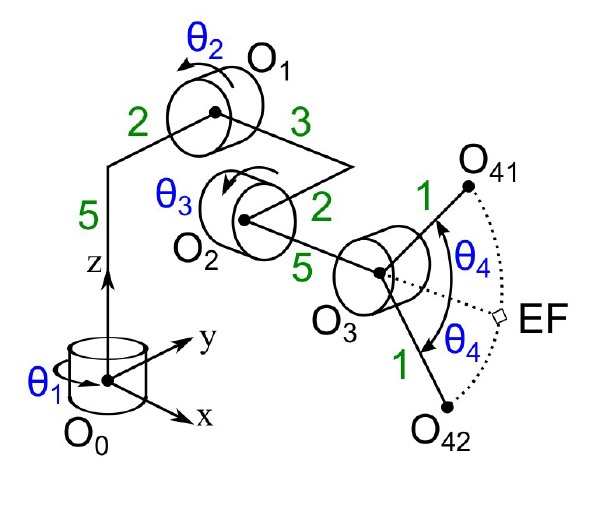
\includegraphics[width=0.8\textwidth]{src/img/Manipulador-5.png}
    \caption{Representación gráfica del manipulador número 5}
    \label{fig:robot5}
\end{figure}

\subsection{Implementación de la cinemática directa del robot número 5}

Tras la visualización del robot número 5 en la figura \ref{fig:robot5}, se procede a realizar la implementación de la cinemática directa del robot. Para ello, se va a utilizar el script en \emph{Python} adjunto en el apartado anterior, modificando los parámetros de la tabla Denavit Hartenberg de la siguiente forma:

\begin{table}[htbp]
  \centering
  \caption{Parámetros D-H}
  \begin{tabular}{|c|c|c|c|c|}
      \hline
      \textbf{Articulación} & $\mathbf{d_i}$ & $\mathbf{\theta_i}$ & $\mathbf{a_i}$ & $\mathbf{\alpha_i}$ \\
      \hline
      05 & 5 & $p[0]$ & 0 & -90 \\
      1 & 2 & 0 & 0 & 0 \\
      15 & 0 & $p[1]$ & 3 & 0 \\
      2 & -2 & -90 & 0 & -90 \\
      3 & 5 & $p[2]$ & 0 & 90 \\
      41 & 0 & $-p[3] + 90$ & 1 & 0 \\
      42 & 0 & $p[3] + 90$ & 1 & 0 \\
      ef & 0 & 90 & 1 & 0 \\
      \hline
  \end{tabular}
\end{table}

Una vez se tienen modificados los parámetros de la tabla, se procede a la modificación del número de manipuladores permitidos por el script, de tal manera que finalmente este toma el siguiente aspecto:

\lstinputlisting[style=python, caption={Script de Cinemática Directa del Manipulador 5}, label=python_script]{src/scripts/Manipulador-5.py}

\section{Ejecución del código}

Para la ejecución del código, se debe ejecutar el siguiente comando en la terminal:

\begin{lstlisting}[style=bash, caption={Ejecución del script de Cinemática Directa del Manipulador 5}, label=bash]
  $  python3 Manipulador-5.py 10 20 30 30
\end{lstlisting}

Tras esto, se obtiene el siguiente resultado:

\begin{figure}[H]
    \centering
    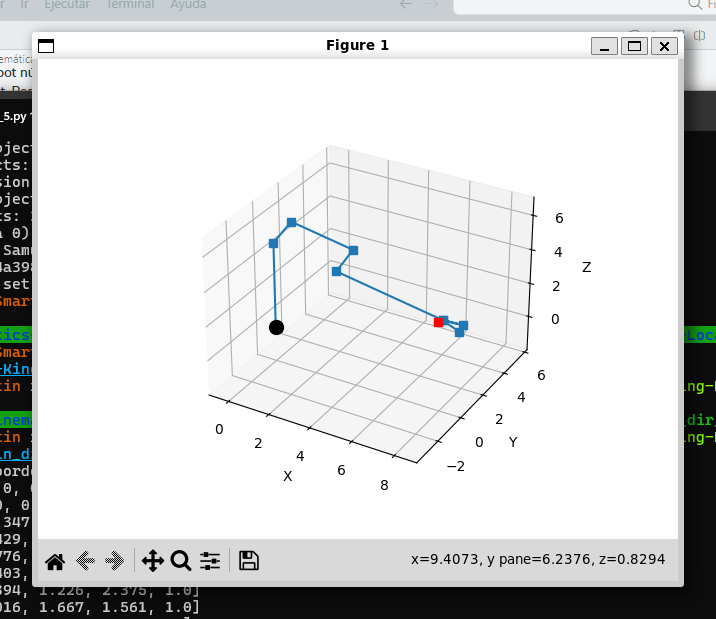
\includegraphics[width=0.8\textwidth]{src/img/Manipulador-5-resultado.png}
    \caption{Resultado de la ejecución del script de Cinemática Directa del Manipulador 5}
    \label{fig:robot5-result}
\end{figure}

\section{Parámetros modificados}

Los parámetros modificados en la implementación de la cinemática directa del robot número 5 han sido los siguientes:

\begin{itemize}
    \item \textbf{Distancia $d_i$}: Se ha modificado el valor de la distancia $d_i$ de la articulación 05, de tal manera que se ha cambiado de 0 a 5.
    \item \textbf{Ángulo $\theta_i$}: Se ha modificado el valor del ángulo $\theta_i$ de la articulación 05, de tal manera que se ha cambiado de 0 a $p[0]$.
    \item \textbf{Ángulo $\alpha_i$}: Se ha modificado el valor del ángulo $\alpha_i$ de la articulación 05, de tal manera que se ha cambiado de 0 a -90.
    \item \textbf{Distancia $d_i$}: Se ha modificado el valor de la distancia $d_i$ de la articulación 1, de tal manera que se ha cambiado de 0 a 2.
    \item \textbf{Ángulo $\theta_i$}: Se ha modificado el valor del ángulo $\theta_i$ de la articulación 1, de tal manera que se ha cambiado de 0 a 0.
    \item \textbf{Distancia $a_i$}: Se ha modificado el valor de la distancia $a_i$ de la articulación 15, de tal manera que se ha cambiado de 0 a 3.
    \item \textbf{Ángulo $\alpha_i$}: Se ha modificado el valor del ángulo $\alpha_i$ de la articulación 15, de tal manera que se ha cambiado de 0 a 0.
    \item \textbf{Distancia $d_i$}: Se ha modificado el valor de la distancia $d_i$ de la articulación 2, de tal manera que se ha cambiado de 0 a -2.
    \item \textbf{Ángulo $\theta_i$}: Se ha modificado el valor del ángulo $\theta_i$ de la articulación 2, de tal manera que se ha cambiado de 0 a -90.
    \item \textbf{Ángulo $\alpha_i$}: Se ha modificado el valor del ángulo $\alpha_i$ de la articulación 2, de tal manera que se ha cambiado de 0 a -90.
    \item \textbf{Distancia $d_i$}: Se ha modificado el valor de la distancia $d_i$ de la articulación 3, de tal manera que se ha cambiado de 0 a 5.
    \item \textbf{Ángulo $\theta_i$}: Se ha modificado el valor del ángulo $\theta_i$ de la articulación 3, de tal manera que se ha cambiado de 0 a $p[2]$.
    \item \textbf{Ángulo $\alpha_i$}: Se ha modificado el valor del ángulo $\alpha_i$ de la articulación 3, de tal manera que se ha cambiado de 0 a 90.
    \item \textbf{Ángulo $\theta_i$}: Se ha modificado el valor del ángulo $\theta_i$ de la articulación 41, de tal manera que se ha cambiado de 0 a $-p[3] + 90$.
    \item \textbf{Ángulo $\theta_i$}: Se ha modificado el valor del ángulo $\theta_i$ de la articulación 42, de tal manera que se ha cambiado de 0 a $p[3] + 90$.
    \item \textbf{Ángulo $\theta_i$}: Se ha modificado el valor del ángulo $\theta_i$ de la articulación ef, de tal manera que se ha cambiado de 0 a 90.
    \item \textbf{Ángulo $\alpha_i$}: Se ha modificado el valor del ángulo $\alpha_i$ de la articulación ef, de tal manera que se ha cambiado de 0 a 0.
    \item \textbf{Distancia $a_i$}: Se ha modificado el valor de la distancia $a_i$ de la articulación ef, de tal manera que se ha cambiado de 0 a 1.
\end{itemize}

Como se puede observar, dependiendo del manipulador que quiera ser implementado, se deben modificar los parámetros de la tabla Denavit Hartenberg de una forma u otra. Es decir, de manera previa, se deben conocer los parámetros de la tabla Denavit Hartenberg del manipulador que se quiere implementar, o en su defecto, como para el caso de la práctica implementada y su modificación, estos valores deben de ser calculados previamente.

\section{Mejoras en la implementación}

Tras la explicación del script de cinemática directa suministrado, se pueden tomar como mejoras de esta práctica pues el hecho de la visualización final del manipulador, es decir, se podría realizar la implementación de la visualización del manipulador en otros tipos de entornos gráficos, como por ejemplo, \emph{Blender}. Es decir, se podría realizar la implementación de la visualización del manipulador en un entorno gráfico más realista, en el cual se podría observar el manipulador en un entorno tridimensional más realista, de tal manera que el alumnado pueda comprender de manera mucho más sencilla y visual el funcionamiento de la cinemática directa mediante Denavit Hartenberg.

Con todo esto comentado, se podría realizar la implementación de la práctica en python de la misma manera que hasta el momento, pero tras la explicación de la matriz de Denavit Hartenberg, se podría trasladar la representación gráfica de python mediante el empleo de la biblioteca \emph{matplotlib} a un entorno gráfico más realista como \emph{Blender}, haciendo uso de librerías como \emph{bpy} \cite{6}.


\section{Conclusiones}

Para concluir con la práctica de Cinemática Directa mediante Denavit Hartenberg, se puede decir que se ha conseguido realizar la implementación de la cinemática directa de un robot manipulador mediante el empleo de la representación de Denavit Hartenberg. Además, se ha conseguido realizar la implementación de la visualización del robot manipulador en un entorno gráfico mediante el empleo de la biblioteca \emph{matplotlib}. Pero, como persona a la que le gusta el mundo de la robótica, me hubiera gustado realizar la implementación de la visualización del robot manipulador en un entorno gráfico más realista como \emph{Blender}, o poder ver su funcionamiento dentro de un manipulador real, ya sea como explicación de la práctica por parte del profesorado, pero, me faltó como esa emoción de poder ver el resultado de la práctica en la realidad.

\chapter{Cinemática inversa}

\section{¿Qué es la Cinemática Inversa?}

Mientras que la cinemática directa se ocupa de calcular la posición y orientación del extremo del robot dado un conjunto de parámetros de articulación, la \emph{cinemática inversa} implica encontrar las configuraciones de las articulaciones necesarias para alcanzar una posición y orientación del extremo. La cinemática inversa es un problema más difícil que la cinemática directa, ya que puede haber más de una solución posible, o ninguna. Además, la cinemática inversa puede ser más difícil de calcular que la cinemática directa, ya que puede requerir la resolución de una ecuación no lineal.

La cinemática inversa es esencial en la programación de robots ya que permite determinar cómo deben moverse las articulaciones para lograr una tarea específica.

\section{Explicación del código suministrado}

El script en python suministrado para la implementación de la práctica de cinemática inversa se puede observar a continuación:

\lstinputlisting[style=python, caption={Script de Cinemática Inversa}, label=python_script]{src/scripts/Inverse-Kinematics-script.py}

Como se puede ver en el script adjunto anteriormente, se realiza la implementación de un script genérico que permite realizar el cálculo de la cinemática inversa de un robot mediante el método de Cierre de Cadena Cinemática (CCD). El método CCD es un algoritmo iterativo que comienza con una estimación inicial de la configuración de las articulaciones y luego mejora la estimación en cada iteración. El algoritmo CCD se puede resumir en los siguientes pasos:

\begin{enumerate}
    \item Seleccionar un punto de destino para el extremo del robot.
    \item Para cada articulación, comenzando con la articulación más alejada del extremo del robot, calcule el vector desde la articulación hasta el punto de destino.
    \item Calcule el vector desde la articulación hasta el extremo del robot.
    \item Calcule el ángulo entre estos dos vectores.
    \item Gire la articulación por este ángulo.
    \item Repita los pasos 2 a 5 hasta que el extremo del robot esté lo suficientemente cerca del punto de destino.
    \item Repita los pasos 1 a 6 para cada punto de destino.
    \item Repita los pasos 1 a 7 hasta que el robot alcance su posición final.
    \item Repita los pasos 1 a 8 para cada posición final.
    \item Repita los pasos 1 a 9 hasta que el robot complete su trayectoria.
\end{enumerate}

Después de definir el algoritmo CCD, se determinan las funciones para mostrar orígenes de coordenadas y representar gráficamente el robot, el programa establece valores iniciales arbitrarios para las articulaciones y longitudes de eslabones. El usuario proporciona las coordenadas del punto objetivo, y utilizando la cinemática directa se calcula la posición inicial y se inicia un bucle iterativo para ajustar las articulaciones de manera que el extremo del robot se acerque al objetivo. En cada iteración, se muestra la posición actual, los orígenes de coordenadas y la distancia al objetivo. Las iteraciones continúan hasta que se alcanza un umbral de convergencia o se supera un límite predefinido de iteraciones.

Finalmente, se presentan los resultados, incluyendo la cantidad de iteraciones necesarias, el umbral de convergencia, la distancia al objetivo y lo valores finales de las articulaciones.

\section{Implementación de la Cinemática Inversa}

Tras la explicación del funcionamiento del script de \emph{cinemática inversa} proporcionado, se realiza la implementación de esta de la siguiente manera:

\lstinputlisting[style=python, caption={Script de Cinemática Inversa implementado de manera correcta}, label=python_script]{src/scripts/Inverse-Kinematics-result.py}

Para comenzar con los cambios realizados dentro del script que se puede observar anteriormente, se realiza la implementación de la cinemática inversa donde se presenta un bucle iterativo basado en el método de Cierre de Cadena Cinemática (CCD) para calcular la cinemática inversa. El bucle continúa hasta que la distancia entre la posición actual del extremo del robot y el objetivo sea menor que un umbral de convergencia (EPSILON). Durante cada iteración, se ajustan las articulaciones del robot para acercar el extremo al objetivo.

El proceso iterativo incluye las siguientes etapas:

\begin{enumerate}
    \item Se almacena la distancia actual como referencia (prev) para evaluar la convergencia.
    \item Para cada articulación, se calcula la cinemática inversa, tomando en cuenta si la articulación es prismática o rotacional.
    \begin{enumerate}
        \item En el caso de una articulación prismática, se ajusta la longitud del eslabón y se normaliza si excede los límites.
        \item Para articulaciones rotacionales, se determina el ángulo de ajuste necesario y se normaliza si es necesario.
    \end{enumerate}
    \item Se actualiza la posición del robot después de cada ajuste.
\end{enumerate}

Tras la implementación de la cinemática inversa, se procede a la inclusión de una función nueva dentro del script, denominada 
como \emph{read\_input\_file}, la cual permite la lectura de un fichero de texto, en el cual se encuentran los valores de los 
distintos parámetros como el tipo de brazo, sus ángulos, los limites superiores, los límites inferiores. Un ejemplo de este 
fichero de texto se puede observar a continuación:

\lstinputlisting[style=bash, caption={Ejemplo de fichero de entrada}, label=example_file]{src/scripts/example-of-type-file-inverse-kinematics.txt}

Finalmente como último cambio realizado al script de cinemática inversa, se realiza la implementación de un \emph{\textbf{menú de ayuda}} que permite al usuario conocer los parámetros que se deben introducir para la ejecución del script, junto con la forma de ejecutar el script.

\section{Ejecución del código}

Tras la explicación de la implementación de la cinemática inversa, se procede a la ejecución del script para la comprobación del funcionamiento del mismo. Para ello, se ejecuta el siguiente comando en la terminal:

\begin{lstlisting}[style=bash, caption={Ejecución del script de Cinemática Inversa}, label=bash]
  $  python3 Inverse-Kinematics-result.py  input-file.txt 15 -10
\end{lstlisting}

Tras esto, se obtiene el siguiente resultado:

\begin{figure}[H]
    \centering
    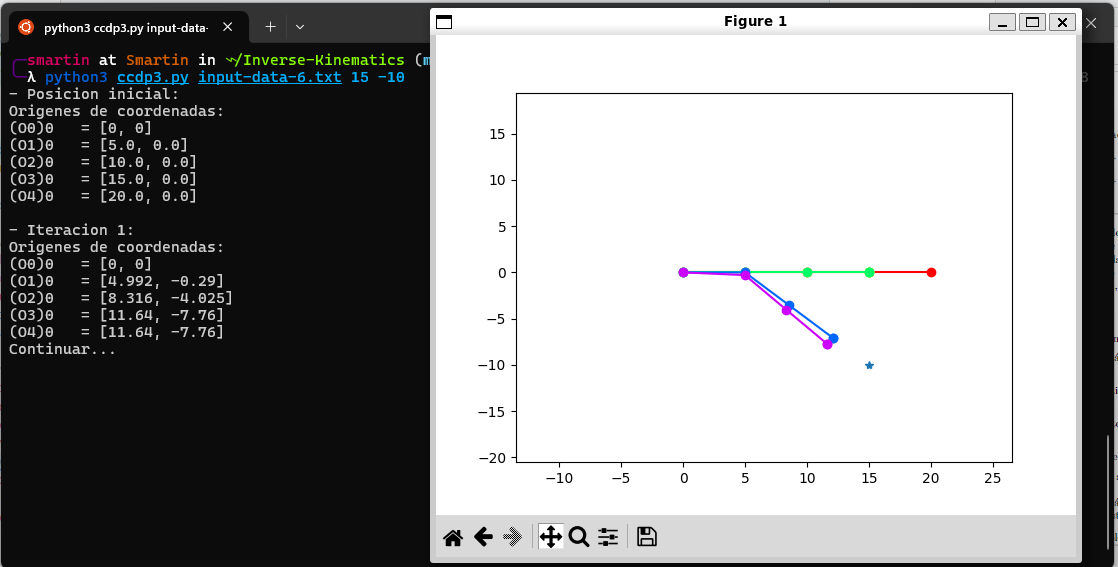
\includegraphics[width=0.9\textwidth]{src/img/Inverse-Kinematics-result.png}
    \caption{Resultado de la ejecución del script de Cinemática Inversa}
    \label{fig:inverse-kinematics-result}
\end{figure}

\section{Parámetros modificados}

Para la implementación de cinemática inversa, se han realizado numerosas pruebas con los parámetros que existen dentro de los ficheros de entrada del programa, es por ello que se han realizado numerosas pruebas con los cambios que se producirían si por ejemplo si se realizan cambios en el tipo de articulación que existe en el brazo, es decir, 0 si se trata de una articulación rotacional y 1 si se trata de una articulación prismática. 

Además, se han realizado pruebas con los cambios que se producirían si se modifican los valores en los \emph{límites superiores} e \emph{inferiores} de las articulaciones, es decir, si se cambian los valores de los límites superiores e inferiores de las articulaciones, se producen cambios en el resultado final de la cinemática inversa. Por último, se han realizado pruebas con los ángulos de las articulaciones, es decir, con los valores de \emph{theta} o finalmente con la \emph{longitud} de los distintos eslabones que componen el brazo.

\section{Conclusiones}

Para concluir, se puede decir que se ha conseguido realizar la implementación de la cinemática inversa de un robot manipulador mediante el empleo del método de Cierre de Cadena Cinemática (CCD). Esta práctica me ha resultado personalmente más interesante en cuanto a su desarrollo y en cuanto a su ejecución, ya que el hecho de poder ver como dependiendo de los valores que se le introduzcan a los distintos eslabones del brazo, se pueda alcanzar el objetivo final de manera más rápido o más lenta dependiendo de los valores que se le introduzcan, me ha resultado muy interesante. Además, cabe destacar que en cuanto a esta práctica no se me ha ocurrido ninguna mejora, ya que la forma de ver como se desplaza el brazo mediante la librería de \emph{matplotlib}, me parece que de esta manera es mucho más cómoda y sencilla de entender y comprender el funcionamiento de la cinemática inversa.

\chapter{Localización}

\section{¿Qué es la localización?}

La localización es el problema de estimar el estado de un robot en un entorno desconocido. El estado de un robot incluye su posición y orientación, así como cualquier otra información que pueda ser útil para determinar su comportamiento futuro. La localización es un problema difícil porque el entorno es desconocido y el robot no tiene acceso a información perfecta sobre su estado. En cambio, el robot debe utilizar información parcial y ruidosa para estimar su estado.

La localización de robots móviles consiste en determinar la posición del robot en relación a un mapa dado del entorno. El problema principal de la localización de un robot móvil reside en que su posición no puede ser medida directamente y debe ser inferida de datos sensoriales. Además, una única medición suele ser de manera habitual insuficiente y el robot debe integrar datos a lo largo del tiempo para determinar su posición.

En el caso de la práctica solicitada por la asignatura de \emph{Robótica Computacional}, el robot móvil no tiene datos sensoriales, sino que se establecen una serie de \emph{"balizas"} en el entorno, las cuales permiten al robot móvil conocer su posición en el entorno, además, se hace uso de otro robot móvil denominado como \emph{"robot rea;"}, el cual se encarga de marcar la diferenciación con respecto al robot móvil al que se debe de aplicar la localización cada vez que este se desvíe o se pierda.

\section{Explicación del código suministrado}

El código suministrado para la implementación de la práctica de localización se puede observar a continuación en dos ficheros distintos, el primero de ellos referente a los robots móviles:

\lstinputlisting[style=python, caption={Script de robot móvil para localización}, label=robot_file]{src/scripts/robot-script.py}

En cuanto al segundo de los scripts, se trata del script referente a los cálculos de las distintas operaciones necesarias para la realización de la localización:

\lstinputlisting[style=python, caption={Script de localización}, label=localization_file]{src/scripts/Localization-script.py}

Teniendo en cuenta los script adjuntos anteriormente, este, simula el movimiento de un robot en un entorno bidimensional y visualiza tanto la trayectoria planificada como la trayectoria real seguida por el robot. A continuación, se proporciona una explicación detallada de su funcionamiento:

El script comienza importando módulos esenciales, como sys para la manipulación de variables del intérprete, math para funciones matemáticas, y un módulo llamado robot que contiene la definición de la clase robot.

Se definen varias funciones útiles, como distancia para calcular la distancia euclidiana entre dos puntos, angulo\_rel  para determinar el ángulo relativo entre la posición actual del robot y un punto objetivo, y mostrar para visualizar gráficamente las trayectorias ideales y reales del robot.

A continuación, se establecen constantes como la pose inicial del robot (P\_INICIAL), la velocidad lineal (V\_LINEAL), la velocidad angular (V\_ANGULAR), la resolución temporal en fotogramas por segundo (FPS), y parámetros que afectan el comportamiento del robot.

Se define una serie de trayectorias predefinidas en la lista trayectorias, y el script toma como entrada de usuario un índice que selecciona una de estas trayectorias.

El script inicializa objetos robot para representar al robot en condiciones ideales (ideal) y condiciones reales con ruido (real). Se establecen parámetros de ruido y pose inicial para ambos robots.

La simulación del movimiento del robot se lleva a cabo en un bucle, calculando velocidades lineales y angulares para alcanzar cada punto en la trayectoria. La simulación continúa hasta que la distancia al objetivo es menor que un umbral (EPSILON) o hasta que se alcanza un límite de iteraciones.

Finalmente, se imprimen resultados como el recorrido total, la distancia real al objetivo, y se utiliza la función mostrar para representar gráficamente las trayectorias ideales y reales del robot. Es importante tener en cuenta que la funcionalidad del script depende del módulo robot.

\section{Implementación de la localización}

Tras la explicación del funcionamiento del script de \emph{localización} proporcionado, se realiza la implementación de esta de la siguiente manera:

\lstinputlisting[style=python, caption={Script de localización implementado}, label=localization_file]{src/scripts/Localization-script-implementation.py}

El script ejecuta una serie de trayectorias, cada una definida por una lista de puntos de destino. Durante la simulación, el robot ajusta su posición y orientación para seguir la trayectoria ideal, con la posibilidad de introducir ruido en las mediciones del sensor. Además, se realiza la implementación de localización basada en la comparación de mediciones de sensores con la posición estimada del robot, utilizando un método de búsqueda en una cuadrícula para encontrar la posición más probable. Es decir, cuando se determina que el robot ideal se ha desviado una cierta variación con respecto al robot real, se aplica la localización para determinar la posición del robot real. Esta localización, se encarga de realizar una búsqueda del robot real dentro de una cuadrícula de píxeles, de tal manera que se determina la posición del robot real dentro de la cuadrícula de píxeles.

Al final de la simulación, se genera una representación gráfica de la trayectoria ideal y la trayectoria seguida por el robot. Este script proporciona una herramienta de simulación para evaluar el rendimiento de la localización del robot y su capacidad para seguir trayectorias específicas en un entorno simulado.

\section{Ejecución del código}

Tras la explicación de la implementación de la localización, se procede a la ejecución del script para la comprobación del funcionamiento del mismo. Para ello, se ejecuta el siguiente comando en la terminal:

\begin{lstlisting}[style=bash, caption={Ejecución del script de Localización}, label=bash]
  $  python3 Localization-script-implementation.py 4
\end{lstlisting}

Tras esto, se obtiene el siguiente resultado:

\begin{figure}[H]
    \centering
    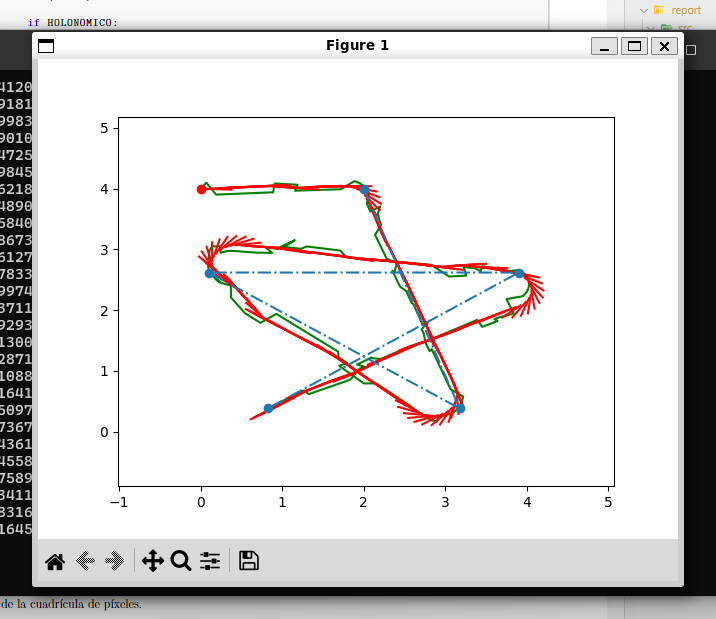
\includegraphics[width=0.8\textwidth]{src/img/Localization-Result.png}
    \caption{Resultado de la ejecución del script de Localización}
    \label{fig:localization-script-implementation}
\end{figure}

\section{Parámetros modificados}

En cuanto a los parámetros modificados durante la implementación de la localización, se pueden tener en cuenta los siguientes parámetros por ejemplo:

\begin{lstlisting}[style=python, caption={Ejecución de la primera operación de Localización}, label=python-script-first-operation]
    localizacion(objetivos,real,ideal, [0, 4],5,1)
\end{lstlisting}

Como se puede observar anteriormente, se pueden modificar los parámetros de \emph{centro}, que para este caso tome como ejemplo \emph{[0, 4]}, los parámetros de \emph{radio}, que para este caso tome como ejemplo \emph{5}. Por tanto, dependiendo de los valores que sean establecidos en estos campos, el resultado de la localización será uno u otro.

Otro de los parámetros con los que se ha jugado un poco ha sido el radio de la localización en el momento en el que se determina que la distancia entre el robot real y el ideal es mayor que un umbral, este valor se puede observar en el trozo de código adjunto a continuación:

\begin{lstlisting}[style=python, caption={Localización del robot}, label=python-robot-localization]
    if (real.measurement_prob(real.sense(objetivos), objetivos) > EPSILON):
        localizacion(objetivos, real, ideal, ideal.pose(), 0.2, mostrar=0)
\end{lstlisting}

Como se puede observar en el trozo de código anterior, se puede modificar el valor del radio de la localización, el cual se encuentra en el campo \emph{0.2}. Cuanto menor sea dicho valor, más preciso será el resultado de la localización, pero, por el contrario, cuanto mayor sea dicho valor, menos preciso será el resultado de esta.

\section{Mejoras en la implementación}

Tras la explicación del script de localización suministrado, se pueden tomar como mejoras de esta práctica pues el hecho de la visualización final del robot, es decir, se podría realizar la implementación de la visualización del robot en otros tipos de entornos gráficos, como por ejemplo, \emph{Blender}. Es decir, se podría realizar la implementación de la visualización del robot en un entorno gráfico más realista, en el cual se pueda observar al robot desplazarse en tiempo real, y no mediante una serie de imágenes estáticas, de tal manera que el alumnado pueda comprender de manera mucho más sencilla y visual el funcionamiento de la localización, es decir, tener tanto al robot real como al robot ideal en tiempo real, de esta manera, cuando se aplique la localización, se pueda observar como el robot real se desplaza hasta la posición del robot ideal.

Para poder conectar los scripts en python con \emph{Blender}, se puede hacer uso de la librería \emph{bpy} \cite{6}, la cual permite la conexión de scripts en python con \emph{Blender}, de tal manera que se podría realizar la implementación de la práctica en python de la misma manera que hasta el momento, pero, cuando se ejecute la operación de localización dentro del script, se pare la visualización en tiempo real de Blender para poder ejecutar una nueva visualización de la localización del robot.

\section{Conclusiones}

Para concluir con la práctica de Localización, se puede decir que se ha conseguido realizar la implementación de la localización de un robot móvil mediante el empleo de una serie de balizas en el entorno, las cuales permiten al robot móvil conocer su posición en el entorno, además, se hace uso de otro robot móvil denominado como \emph{"robot real"}, el cual se encarga de marcar la diferenciación con respecto al robot móvil al que se debe de aplicar la localización cada vez que este se desvíe o se pierda. 

Esta práctica me ha resultado personalmente la más interesante de las tres prácticas realizadas, ya que el hecho de poder ver como dependiendo de los valores que se le introduzcan a los distintos parámetros de la localización, se tenga que el robot sea más preciso o menos, me resulta muy interesante, porque para mi, la localización es una de las partes más importantes de la robótica, ya que si no se tiene una buena localización, el robot no podrá realizar las tareas que se le encomienden de manera correcta.

\chapter{Filtro de partículas}

\section{¿Qué es un filtro de partículas?}

El filtro de partículas es un método de estimación de estado que utiliza una aproximación basada en muestras para representar la distribución de probabilidad de un estado. El filtro de partículas es un método no paramétrico, lo que significa que no hace suposiciones sobre la forma de la distribución de probabilidad. En cambio, el filtro de partículas representa la distribución de probabilidad mediante una colección de muestras, llamadas partículas, que se distribuyen de acuerdo con la distribución de probabilidad. 

La idea fundamental se basa en representar la función de distribución posterior buscada con un conjunto de muestras aleatorias con pesos asociados y calcular estimados basados en estas muestras y pesos.

\begin{thebibliography}{99}
  \bibitem{1} UdeSantigoVirtual. [2023]. Herramientas matemáticas. Universidad de Santiago de Chile. Recuperado de \url{http://www.udesantiagovirtual.cl/moodle2/mod/book/view.php?id=24916}
  \bibitem{2} Samuel Martín Morales. [2023]. Direct-Kinematics-using-Denavit-Hartenberg. GitHub. Recuperado de \url{https://github.com/Samuelmm15/Direct-Kinematics-using-Denavit-Hartenberg.git}
  \bibitem{3} Samuel Martín Morales. [2023]. Inverse-Kinematics. GitHub. Recuperado de \url{https://github.com/Samuelmm15/Inverse-Kinematics.git}.
  \bibitem{4} Samuel Martín Morales. [2023]. Robot-Localization. GitHub. Recuperado de \url{https://github.com/Samuelmm15/Robot-Localization.git}.
  \bibitem{5} Universidad de La Laguna. [2023]. Cinemática Directa mediante Denavit-Hartenberg. Universidad de La Laguna. \url{https://drive.google.com/file/d/1639F9ebw14zquNaZcDf6o_u-_Tpaksh4/view?usp=sharing}
  \bibitem{6} Comunidad Python. [2023]. bpy - Blender Python. Comunidad Python. \url{https://pypi.org/project/bpy/}
  \bibitem{7} Escamilla Losoyo José de Jesús. [2020]. Cinemática inversa. Studocu. \url{https://www.studocu.com/es-mx/document/instituto-tecnologico-de-leon/robotica/cinematica-inversa/12281135}
  \bibitem{8} Tekniker. [2023]. Localización y planificación de trayectorias. Tekniker. \url{https://www.tekniker.es/es/localizacion-y-planificacion-de-trayectorias}
  \bibitem{9} Wikipedia. [2023]. Filtro de partículas. Wikipedia. \url{https://es.wikipedia.org/wiki/Filtro_de_part%C3%ADculas}
  \bibitem{10} Azucena Fuentes Ríos. [2011]. LOCALIZACIÓN Y MODELADO SIMULTÁNEOS
  EN ROS PARA LA PLATAFORMA ROBÓTICA
  MANFRED. Universidad Carlos III de Madrid. \url{https://e-archivo.uc3m.es/bitstream/handle/10016/13392/pfc_Azucena_Fuentes_Rios.pdf?sequence=1&isAllowed=y}
\end{thebibliography}

\end{document}